\chapter{Modelling}

\section{Mass determination of Omega Centauri}

We used various techniques for the determination of the dynamic and stellar mass of NGC5139 that we use to model the mass more accurately. 

\subsection{Stellar Population Synthesis with Starlight}

The stellar mass content of Globular Clusters and Galaxies can be studied through the determination of the stellar populations inside those systems since we have clear knowledge about their photometric properties. If we have information about the amount of stars of a given type inside a stellar system, we can infer how much of the system's mass is given by these populations of stars. 

The determination of the stellar populations can be done using STARLIGHT, which is a Fortran-based program that fits an observed integrated spectrum (Omega Centauri in our case) with a model spectrum which is the sum of $N_{*}$ spectral components from a pre-defined and pre-processed set of base spectra. The program does as many iterations as the user decides to sum up the different template spectra until a good fitting of the spectral lines has been made to the observed spectrum. 

The output of the program after the execution contains the created spectrum (wavelength and intensity) and the approximate percentage of each of the stellar population inside the stellar system. Since the stellar populations are well documented the output will also contain the metallicity of each of them so that further analysis can be made upon STARLIGHT's results.

First, one must prepare the observed spectrum before running STARLIGHT, the spectrum has to be wavelength and flux calibrated, taking into account the bad-pixel removal. Very importantly in the context of mass analysis, the spectrum has to be extinction corrected so that the units of flux relate properly to the units if the templates in STARLIGHT.     

The extinction correction for our observed spectrum is given by

\begin{equation}
f_{obs}(\lambda)=f_{int}(\lambda)10^{-0.4A_{\lambda}}
\end{equation}

Where $A_{\lambda}=0.213$ in the I filter around $8000 \textrm{\AA}$, around the wavelength range of our spectrum. 

On our case, we have to multiply by a factor of 1.216746 the intensity of the spectrum for the flux calibration to be made. After we apply the extinction correction to the spectrum and create an ASCII table with the wavelength, intensity and error columns, it is now ready to be processed with STARLIGHT as we can see in the following figure:

\begin{figure}[H]
\centering
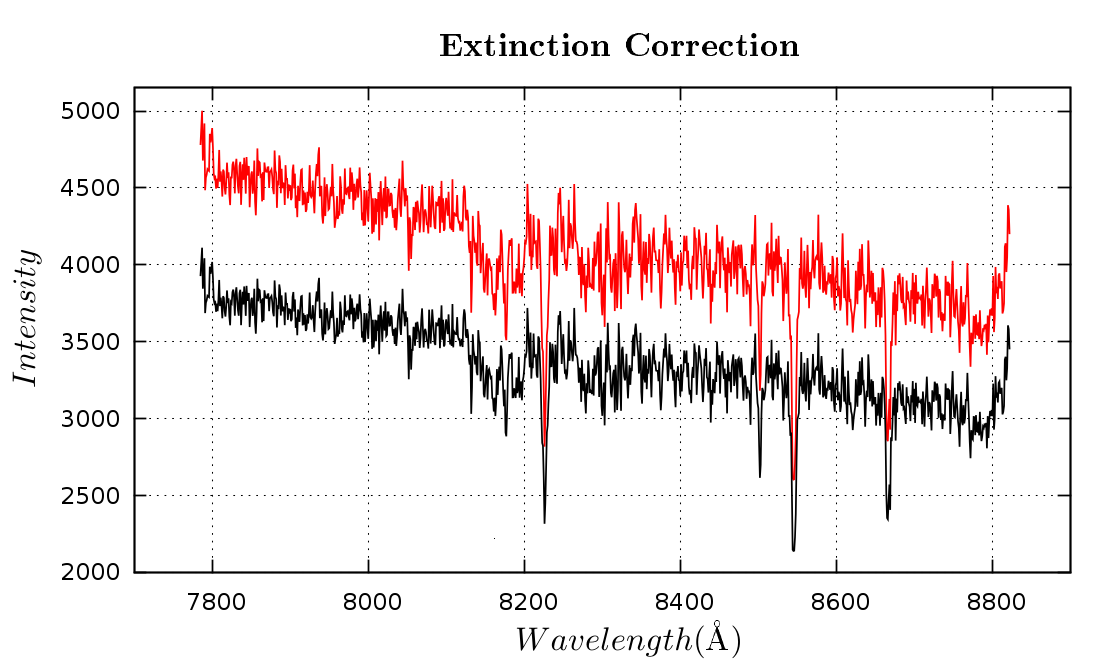
\includegraphics[width=10cm]{images/extinction.png}
\caption[Extinction Correction]{This figure shows an integrated spectrum of the central region of Omega Centauri before and after the extinction correction is applied. The black line has the original flux values and the black line has the corrected flux, that is, the flux that would be observed if there wasn't any interstellar medium that obscures the light coming from the object.}
\end{figure}

Before running STARLIGHT one must assure that the wavelength range is correctly specified in the configuration file that also includes the database of the template spectra and the bad data organized in a mask file. When all of these is ready it is staightforward to run STARLIGHT with the following command:

\begin{center}
./StarlightChains\_v04.exe $<$ Omega\_cen.in
\end{center}

The synthetic spectrum and the original one look like this:

\begin{figure}[H]
\centering
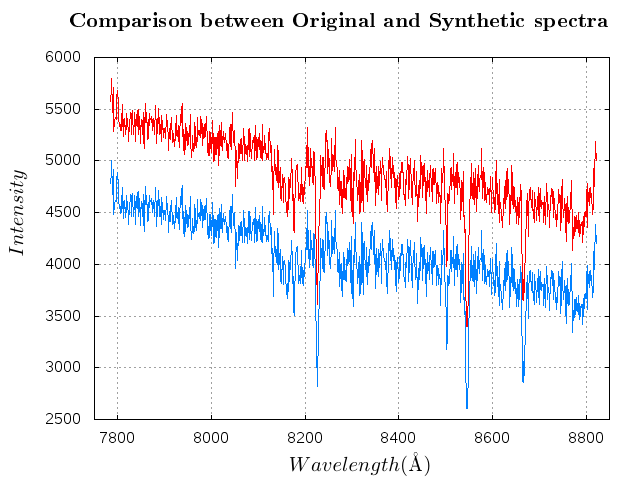
\includegraphics[width=10cm]{images/comparison.png}
\caption[Synthetic spectrum of STARLIGHT]{Synthetic spectrum of Starlight in red, shifted in the y axis for doing the comparison with the original spectrum of Omega Centauri in blue.}
\end{figure}
 
Now, besides the synthetic spectrum, the output file contains some useful results that one can use to calculate the mass of the stellar system. In our case, the relevant parameter that STARLIGHT gives is:

\begin{equation}
Mcor\_tot = 3.29446 \times 10^{7}
\end{equation}

And using the formula:

\begin{equation}
M_{\star}=Mcor\_tot\times10^{-17}\times4\pi d^{2}\times\left(3.826\times10^{33}\right)^{-1}
\end{equation}

Yields a stellar mass of $M_{\star}=243.462M_{\odot}$

This mass is the stellar mass contained in the detection area (that in our set up configuration in OPD ends up to be $A_{D}=0.36\,pc^{2}$) of the integrated spectrum that we analysed with STARLIGHT so if we want to calculate the whole stellar mass of the Globular system we must extrapolate this result to its whole effective area, noting that this will increase the error of the calculation.

If we take the cluster's tidal radius to be 45' (Trager et al. 1995) and it's distance to the sun of $4808.39\,pc$ then the total effective area (where the stellar mass could be calculated using stellar population synthesis) is $A_{OC}=12445.9\,pc^{2}$. 

Finally, the total stellar mass of the Cluster using this technique can be calculation using:

\begin{equation}
M_{\star T} = N \times M_{\star}
\end{equation}

Where N is the number of detection areas within the total effective area of Omega Centauri ($A_{OC}/A_{D}$) of about 31844.8. So that our calculation of the stellar mass is finally:

\begin{equation}
M_{\star T} = 6.2734 \times 10^{6}M_{\odot}
\end{equation}
 
This result is actually higher than some values  of the dynamical mass found in the literature:

\begin{table}[H]
\begin{center}
  \begin{tabular*}{0.55\textwidth}{@{\extracolsep{\fill} } |  c | c | }
    \hline
    \textbf{Paper} & \textbf{Mass} \\ \hline
    Van de Ven et al. 2008 & $\sim 2.5 \times 10^{6} M_{\odot}$ \\
    Mandushev et al. 1991 & $\sim 2.4 \times 10^{6} M_{\odot}$ \\
    Meylan et al. 1995 & $\sim 5.1 \times 10^{6} M_{\odot}$ \\
    Jalali et al. 2011 & $\sim 2.5 \times 10^{6} M_{\odot}$ \\
    \hline
  \end{tabular*}
\end{center} 
\caption[Mass Omega Centauri]{Reported values of Omega Centauri's dynamical mass}
\end{table}

The stellar mass should in principle, by smaller or at least equals to the dynamical mass, this discrepancy in our first approach to the mass determination is probably due to errors given by the extrapolation of the results of the detection area to the whole area of the cluster, because our detection area was very small ($\sim 0.2 \, arcmin^{2}$) compared to the cluster's size of more than $6,000 \, arcmin^{2}$. Still, the stellar population technique is consistent with the order of magnitude of the cluster's mass previously reported.  

\subsection{Modified Hernquist Model}

\subsection{Color-Magnitude diagrams}

